\ifx\allfiles\undefined
\documentclass[12pt, a4paper, oneside, UTF8]{ctexbook}  %  这一句是新增加的
\usepackage[dvipsnames]{xcolor}
\usepackage{amsmath}   % 数学公式
\usepackage{graphicx}
\usetikzlibrary{arrows, calc, decorations.pathmorphing}
\allowdisplaybreaks % 允许公式跨页换行
\newcommand{\pa}{\partial}
\newcommand{\mathminus}{\!\!-\!\!} % 数学环境连字符
\newcommand{\vsup}[1]{\raisebox{-0.1ex}{$\scriptstyle #1$}}
\newcommand{\lsup}[1]{\raisebox{-0.85ex}{$\scriptstyle #1$}}
\definecolor{b1}{RGB}{0,191,255}



\begin{document}
%
 % 单独编译时,其实不用编译封面目录之类的,如需要不注释这句即可
\else
\fi
%  ↓↓↓↓↓↓↓↓↓↓↓↓↓↓↓↓↓↓↓↓↓↓↓↓↓↓↓↓ 正文部分
\chapter{concise review of basic concepts and definitions}
\section{class 1}
\begin{defn}
\par\indent
\begin{enumerate}
    \item \textcolor{b1}{system}:\;
    set of constituents\;(\textbf{not subjected to forces that depend on coordinates of other external constituents})
    \item \textcolor{b1}{property}:\; 
    the system at time \( t \), yields a numerical result \( P(t) \)\;(\textbf{not depend on other instants of time})
    \item \textcolor{b1}{state}:\; 
    the state of the system at time \( t \) is the set of
     (a) the values of the amounts of all constituents,
     (b) the values of the external and internal, and
     (c) the values of all the conceivable properties
\[ A(t) = \{ n_1(t), \cdots, n_r(t), \beta_1(t), \cdots, \beta_s(t), P_1(t), P_2(t), \cdots \} 
\qquad A_1:=A(t_1)\]
\begin{itemize}
    \item \( r\) number of different constituents
    \item \( s\) number of parameters
\end{itemize}
\begin{add}
    Time evolution of the state of the system
    General equation of motion:
\[ \frac{dA(t)}{dt} = f[A(t), \text{forces}(t)] \rightarrow A(t_1)\]

Two theorems of the equation of motion hold for all (well-defined) systems:
\begin{enumerate}
\item First Theorem (Conservation of Linear Momentum)
\item Second Theorem (Conservation of Angular Momentum)
\end{enumerate}
\begin{zhu}
    "well-defined systems"(良好定义的系统)指的是那些能够用明确的数学框架(如拉格朗日力学或哈密顿力学)来描述的系统。
\end{zhu}
\end{add}
    \item \textcolor{b1}{process}:\; 
    specified by
    \begin{itemize}
    \item The initial state of the system
    \item The final state of the system
    \item The effects produced by the interactions with other systems
    \end{itemize}
    \[ A_1 \rightarrow A_2 \]
    \begin{zhu}
        A process simplifies the description of time evolution by abstracting the behavior of a system 
        into a series of state changes over time. 
        
        Instead of detailing \textbf{every instantaneous configuration 
        or interaction}, a process focuses on the overall transformation \textbf{from an initial state to a final state}.
    \end{zhu}
\end{enumerate}
\end{defn}
\begin{defn}
    \par\indent
    \begin{itemize}
        \item Spontaneous Process (no effects on the environment)
        \item Weight Process (external effects are only ``mechanical''(mechanical work))
    \end{itemize}
    \begin{zhu}
    \par\indent
\begin{itemize}
    \item Spontaneous Process 强调了热力学中的不可逆性和能量转换的方向性,将力学中的能量概念与热力学中的熵增联系起来。
    \item Weight Process 将力学中的功与热力学中的能量守恒联系起来。
\end{itemize}
    \end{zhu}
\end{defn}
\begin{law}
    First Law (a unique form):
    \begin{itemize}
    \item \textbf{Assertion 1:} any pair of states \( A_1 \) and \( A_2 \) with 
    compatible values of the amounts of constituents and the parameters of 
    a (well-defined) system \( A \) \textbf{can always be interconnected by} means of a weight process.
    \item \textbf{Assertion 2:} the product \( mg(z_2 - z_1) \) assumes \textbf{the same value for all weight processes} that connect the two given states \( A_1 \) and \( A_2 \).
    \end{itemize}
\end{law}
\begin{corollary}
    Consequences of the First Law:
    \begin{enumerate}
        \item Additivity of energy
        \item Conservation of energy
        \item Exchangeability of energy via interactions
        \item Energy balance equation for a process for system \( A \) (the usual form of the First Law)
    \end{enumerate}
\end{corollary}
\begin{minipage}{0.85\textwidth}
    \centering
    \captionof{table}{Comparison of Steady, Unsteady, Equilibrium, and Nonequilibrium States}
    \begin{tabular}{|p{4cm}<{\centering}|p{4cm}<{\centering}|p{5cm}<{\centering}|}
        \hline
            ~ & ...because of external interactions & ...even if external interactions are turned off \\ 
        \hline
            The state changes with time... & Unsteady state  & Nonequilibrium state \\
        \hline
            The state does not change with time... & Steady state  & Equilibrium state \\ 
        \hline
    \end{tabular}
\end{minipage}
\begin{defn}
    Unstable equilibrium,
    Metastable equilibrium,
Stable equilibrium and

Nonequilibrium
    \par\indent
\begin{minipage}{0.8\textwidth}
    \centering
    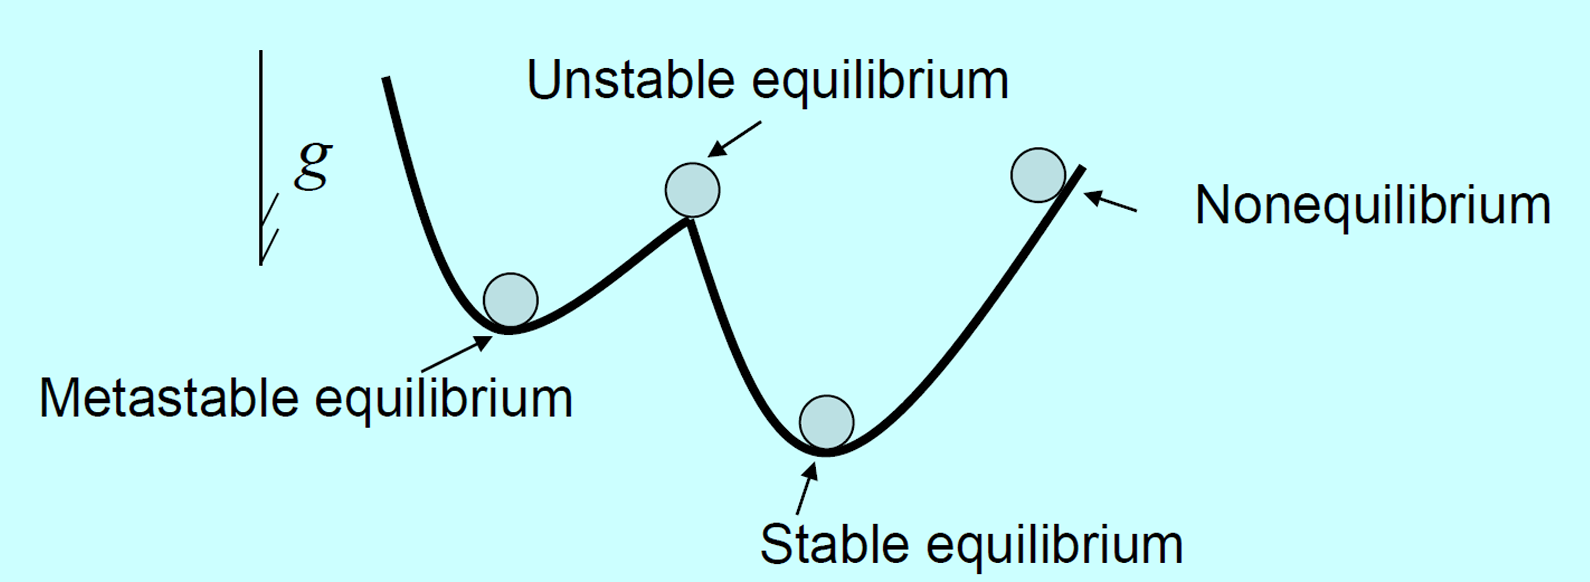
\includegraphics[width=0.75\textwidth]{chap1/1.1.png}
\end{minipage}
\end{defn}
\begin{law}
    Second Law:

\begin{itemize}
\item \textbf{Assertion 1:} in the subset of states of a system compatible with 
given values of the amounts of constituents \( n \) and of the parameters \( \beta \), 
there is always \textbf{one and only one SES} for each value of the energy \( E \).  
\item \textbf{Assertion 2:} Starting from any state of the system, it is always possible, 
\textbf{through a reversible weight process}, to reach a SES with arbitrarily fixed, 
\textbf{compatible values of the amounts} of constituents and the parameters.
\end{itemize}
\begin{zhu}
    \par\indent
    \begin{itemize}
    \item \textbf{Mechanics:} One and only one: the stable equilibrium state with minimum energy, \( E_g (n, \beta) \). 
    \item \textbf{Thermodynamics:} One for every value of the energy \( E \)
\end{itemize}
\end{zhu}
\end{law}
\section{class 2}
\begin{thm}
    Consequences of First \& Second Law Together Entail
    \begin{itemize}
        \item Kelvin-Planck statement: impossibility of perpetual motion of the second kind
        
        (It is impossible to extract mechanical energy without other effects from a system initially in a stable equilibrium state)
        % \item Supports the definition of property adiabatic availability
        % \item Supports the definition of property temperature of a thermal reservoir
        % \item Supports the definition of property entropy
        % \item Principle of nondecrease of entropy. Entropy balance
        % \item Criteria to determine if a process is reversible or not
        % \item State principle and fundamental relation for the stable equilibrium states
        % \item Conditions for mutual equilibrium between systems
        \item Clausius statement: Conditions for the spontaneous exchange of energy between systems initially in stable equilibrium states but not in mutual equilibrium
    \end{itemize}
\begin{proof}
    the Kelvin-Planck Statement of the Second Law

\textbf{Ab absurdo:} assume that a PMM2 be possible (further assume, for simplicity of proof here, 
that system \( A \) is composed of two separate parts).

The final states is different from the initial one, and the initial
one was a Steady Equilibrium State.
\end{proof}
\begin{zhu}
    Synonyms of ab absurdo include “reductio ad absurdum,” “proof by contradiction,” and “proof by absurdity.”
\end{zhu}
\end{thm}
\begin{defn}
    The \textbf{adiabatic availability} \( \Psi_1 \) of system \( A \) in state \( A_1 \) 
    measures \textbf{the maximum amount of energy} that \textbf{can be transferred} from the system 
    to a weight in a weight process for \( A \) starting from state \( A_1 \).
    \(\Psi_1=E_1-E_{s1}\)
\end{defn}
\begin{thm}
    Adiabatic availability is a property, but it is \(\underset{\text{lack of utility}}{\text{not additive}}\).
\end{thm}
\begin{defn}
    Mutual stable equilibrium
      
    Two systems \( A \) and \( B \) are in mutual stable equilibrium if their respective states are such that the composite system \( AB \) is in a stable equilibrium state.
\end{defn}
\begin{defn}
    A system \( R \) that in any of its stable equilibrium states is 
    in mutual equilibrium with a given system \( C \) in a given state \( CR \).
    \begin{explain}
        A thermal reservoir, denoted as \(R\), 
        is a system that can exchange energy (typically heat) with another system 
    \(C\) without undergoing any significant change in its own properties.     
    \end{explain}
    \begin{zhu}
        Thermal reservoirs are often used as heat sources or sinks in thermodynamic processes. 
    \end{zhu}
\end{defn}
\begin{proposition}
    It can be proved that the ratio:
\[ \frac{(E_{s2rev}^R - E_{s1}^R)_{A_1 R_{s1} \underset{w,rev}{\rightarrow} A_2 R_{s2rev}}}
{(E_{s2rev}^{R^\circ } - E_{s1}^{R^\circ })_{A_1 R_{s1}^\circ \underset{w,rev}{\rightarrow} A_2 R^\circ _{s2rev} }} 
\]
\begin{itemize}
    \item is positive, 
    \item is independent of \(\begin{cases}
    \text{the initial states}\; R_{s1}, \;R^\circ_{s1}\; \text{of the reservoirs,}\\
    \text{the choice of the auxiliary system} \;A\; \text{and of its states} \; A_1 \;\text{and}\; A_2 , 
    \end{cases}\)
    \item depends solely on the pair of reservoirs \( R \) and \( R^\circ \),
    \item is a dimensionless number.
\end{itemize}
\end{proposition}
\begin{defn}
    property temperature of reservoir \(R\)
\begin{gather*}
T_R=T_{R^\circ}\frac{(E_{s2rev}^R - E_{s1}^R)_{A_1 R_{s1} \underset{w,rev}{\rightarrow} A_2 R_{s2rev}}}
{(E_{s2rev}^{R^\circ } - E_{s1}^{R^\circ })_{A_1 R_{s1}^\circ \underset{w,rev}{\rightarrow} A_2 R^\circ _{s2rev} }} 
\\
\frac{(E_{s2rev}^R - E_{s1}^R)_{A_1 R_{s1} \underset{w,rev}{\rightarrow} A_2 R_{s2rev}}}{T_R}
=\frac{(E_{s2rev}^{R^\circ } - E_{s1}^{R^\circ })_{A_1 R_{s1}^\circ \underset{w,rev}{\rightarrow} A_2 R^\circ _{s2rev}}}{T_{R^\circ}}
\end{gather*}

The ratio 
\begin{itemize}
    \item is independent of reservoir \( R \) and of its initial state \( R_{s1} \)
    \item It depends therefore only on system \( A \) and the pair of states \( A_1 \) and \( A_2 \)
\end{itemize}
\end{defn}
\begin{defn}
    property entropy
    
    The ratio:
\[
\frac{\left(E_{s0\text{rev}}^R - E_{s1}^R\right)_{A_1 R_{s1} \underset{w,rev}{\rightarrow} A_0 R_{s0\text{rev}}}}{T_R}
\]
\begin{itemize}
    \item is independent of reservoir \( R \) and of its initial state \( R_{s1} \)
    \item It depends therefore only on system \( A \) and the pair of states \( A_1 \) and \( A_0 \)
\end{itemize}
\[
S_1 = S_0 + \frac{\left(E_{s0\text{rev}}^R - E_{s1}^R\right)_{A_1 R_{s1} \underset{w,rev}{\rightarrow} A_0 R_{s0\text{rev}}}}{T_R}
\]
\end{defn}
















%  ↑↑↑↑↑↑↑↑↑↑↑↑↑↑↑↑↑↑↑↑↑↑↑↑↑↑↑↑ 正文部分
\ifx\allfiles\undefined
\end{document}
\fi
